\documentclass[problem]{mcs}

\begin{pcomments}
  \pcomment{FP_simple_graphs_trees_short_answer}
  \pcomment{excerpted from FP_graphs_short_answer, MQ_matching,
      FP_multiple_choice_unhidden, MQ_list_isomorphisms}
  \pcomment{ARM 12/14/15} 

\end{pcomments}

\pkeywords{
  simple_graph
  tree
  isomorphism
  bottle_neck
  chromatic
  complete_graph
}

%%%%%%%%%%%%%%%%%%%%%%%%%%%%%%%%%%%%%%%%%%%%%%%%%%%%%%%%%%%%%%%%%%%%%
% Problem starts here
%%%%%%%%%%%%%%%%%%%%%%%%%%%%%%%%%%%%%%%%%%%%%%%%%%%%%%%%%%%%%%%%%%%%%

\begin{problem} 
Answer the following questions about \textbf{finite simple graphs}.
You may answer with formulas involving exponents, binomial
coefficents, and factorials.

\bparts

\ppart How many edges are there in the \emph{complete graph} $K_{41}$?
\hfill \examrule

\begin{solution}
\[
\binom{41}{2} = 820.
\]
\end{solution}

\ppart How many edges are there in a spanning tree of $K_{41}$? \hfill \examrule

\begin{solution}
\textbf{40}.
\end{solution}

\ppart What is the chromatic number $\chi(K_{41})$? \hfill \examrule
\begin{solution}
41.
\end{solution}

\ppart What is the chromatic number $\chi(C_{41})$, of the cycle of
  length 41? \hfill \examrule

\begin{solution}
\textbf{3}.
\end{solution}

\ppart Let $G$ be the graph in Figure~\ref{graphs_for_isomorphism_a}.
How many distinct isomophisms are there from $G$ to $G$?
\hfill \examrule

\begin{figure}[h]
\graphic[height=0.75in]{isomorphism_a}
\caption{The graph $G$}
\label{graphs_for_isomorphism_a}
\end{figure}

\begin{solution}
\textbf{4}.
\end{solution}

\ppart How many cycles can there be in a graph created by adding a
single edge\\
to a tree with 41 vertices?  \hfill \examrule

\begin{solution}
Exactly \textbf{1}.
\end{solution}

\ppart What is the smallest number of leaves possible in a tree with
41 vertices? \hfill \examrule
\begin{solution}
\textbf{2}.
\end{solution}

\ppart What is the largest possible number of leaves possible in a
tree with 41 vertices? \hfill \examrule
\begin{solution}
\textbf{40}.
\end{solution}

\ppart How many trees are there whose vertices are the integers
$\Zintv{1}{41}$? \hfill \examrule
\begin{solution}
$41^{39}$.  See Problem~(\bref{CP_numbered_trees}).
\end{solution}

\ppart Show that there is no perfect matching for the bipartite graph
$H$ in Figure~\ref{fig:bipartite_with_bneck} by listing the vertices
in a set that forms a \emph{bottleneck}.  (You may choose vertices
from $\rightbi{H}$ or from $\leftbi{H}$.) \hfill \examrule[1.5in]

\begin{figure}[h]
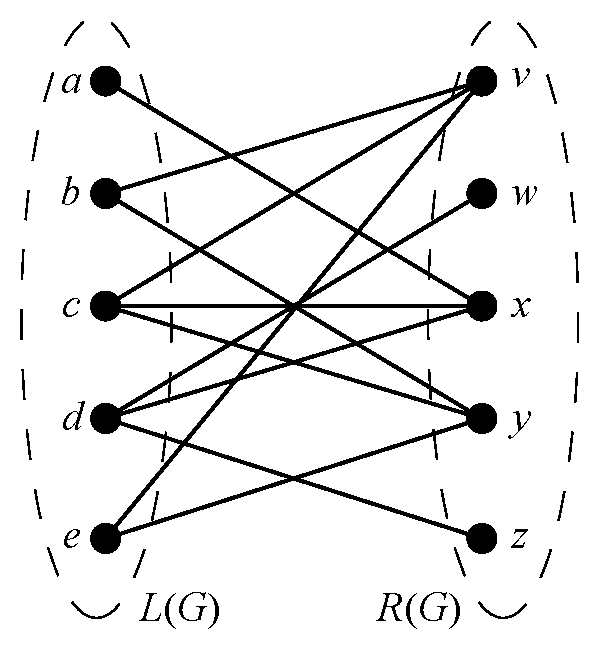
\includegraphics[width=1.5in]{MQ_bipartite_with_bottleneck}
\caption{Bipartite graph $H$}.\label{fig:bipartite_with_bneck}
\end{figure}

\begin{solution}
The set $\set{a,b,c,e}$ is a bottleneck:
\[
\card{H(\set{a,b,c,e})} = \card{\set{v,x,y}} = 3 < 4 = \card{\set{a,b,c,e}}.
\]

The set $\set{w,z}$ is a bottleneck in the other direction:
\[
\card{H^{-1}(\set{w,z})} = \card{\set{d}} = 1 < 2 = \card{\set{w,z}}.
\]
\end{solution}

\ppart How many length 11 cycles are in $K_{41}$? \hfill \examrule

\begin{solution}
\textbf{10!}

 A cycle is determined by the sequence of 11 vertices in it, but since
 a cycle has no ``first'' or ``last'' vertex, 11 different sequences
 determine the same cycle.  So the number of cycles equals the number
 of sequences, namely $11!$ divided by 11.
\end{solution}

\ppart How many cycles can there be in a graph created by adding two\\
edges to a tree with 41 vertices? \hfill \examrule

\begin{solution}
\textbf{2 or 3}.
\end{solution}


\eparts

\end{problem}

\endinput
